% !TEX TS-program = xelatex
% !TEX spellcheck = en-US

%%%%%%%%%%%%%%%%%%%%%%%%%%%%%%%%%%%%%%%%%
% Twenty Seconds Resume/CV
% LaTeX Template
% Version 1.0 (14/7/16)
%
% Original author:
% Carmine Spagnuolo (cspagnuolo@unisa.it) with major modifications by
% Vel (vel@LaTeXTemplates.com) and Harsh (harsh.gadgil@gmail.com)
%
% License:
% The MIT License (see included LICENSE file)
%
%%%%%%%%%%%%%%%%%%%%%%%%%%%%%%%%%%%%%%%%%

% XeLaTex

%----------------------------------------------------------------------------------------
%  PACKAGES AND OTHER DOCUMENT CONFIGURATIONS
%----------------------------------------------------------------------------------------

\documentclass[a4paper]{twentysecondcv} % a4paper for A4

\usepackage{hyperref}
\hypersetup{
pdftitle={John Paul Newman CV},
pdfsubject={CV},
pdfauthor={John Paul Newman},
pdfkeywords={CV}
}

%%% Configure a directory location for sections
\newcommand*{\sectiondir}{sections/}

% Command for printing skill overview
\newcommand\skills{
\vspace{4mm}
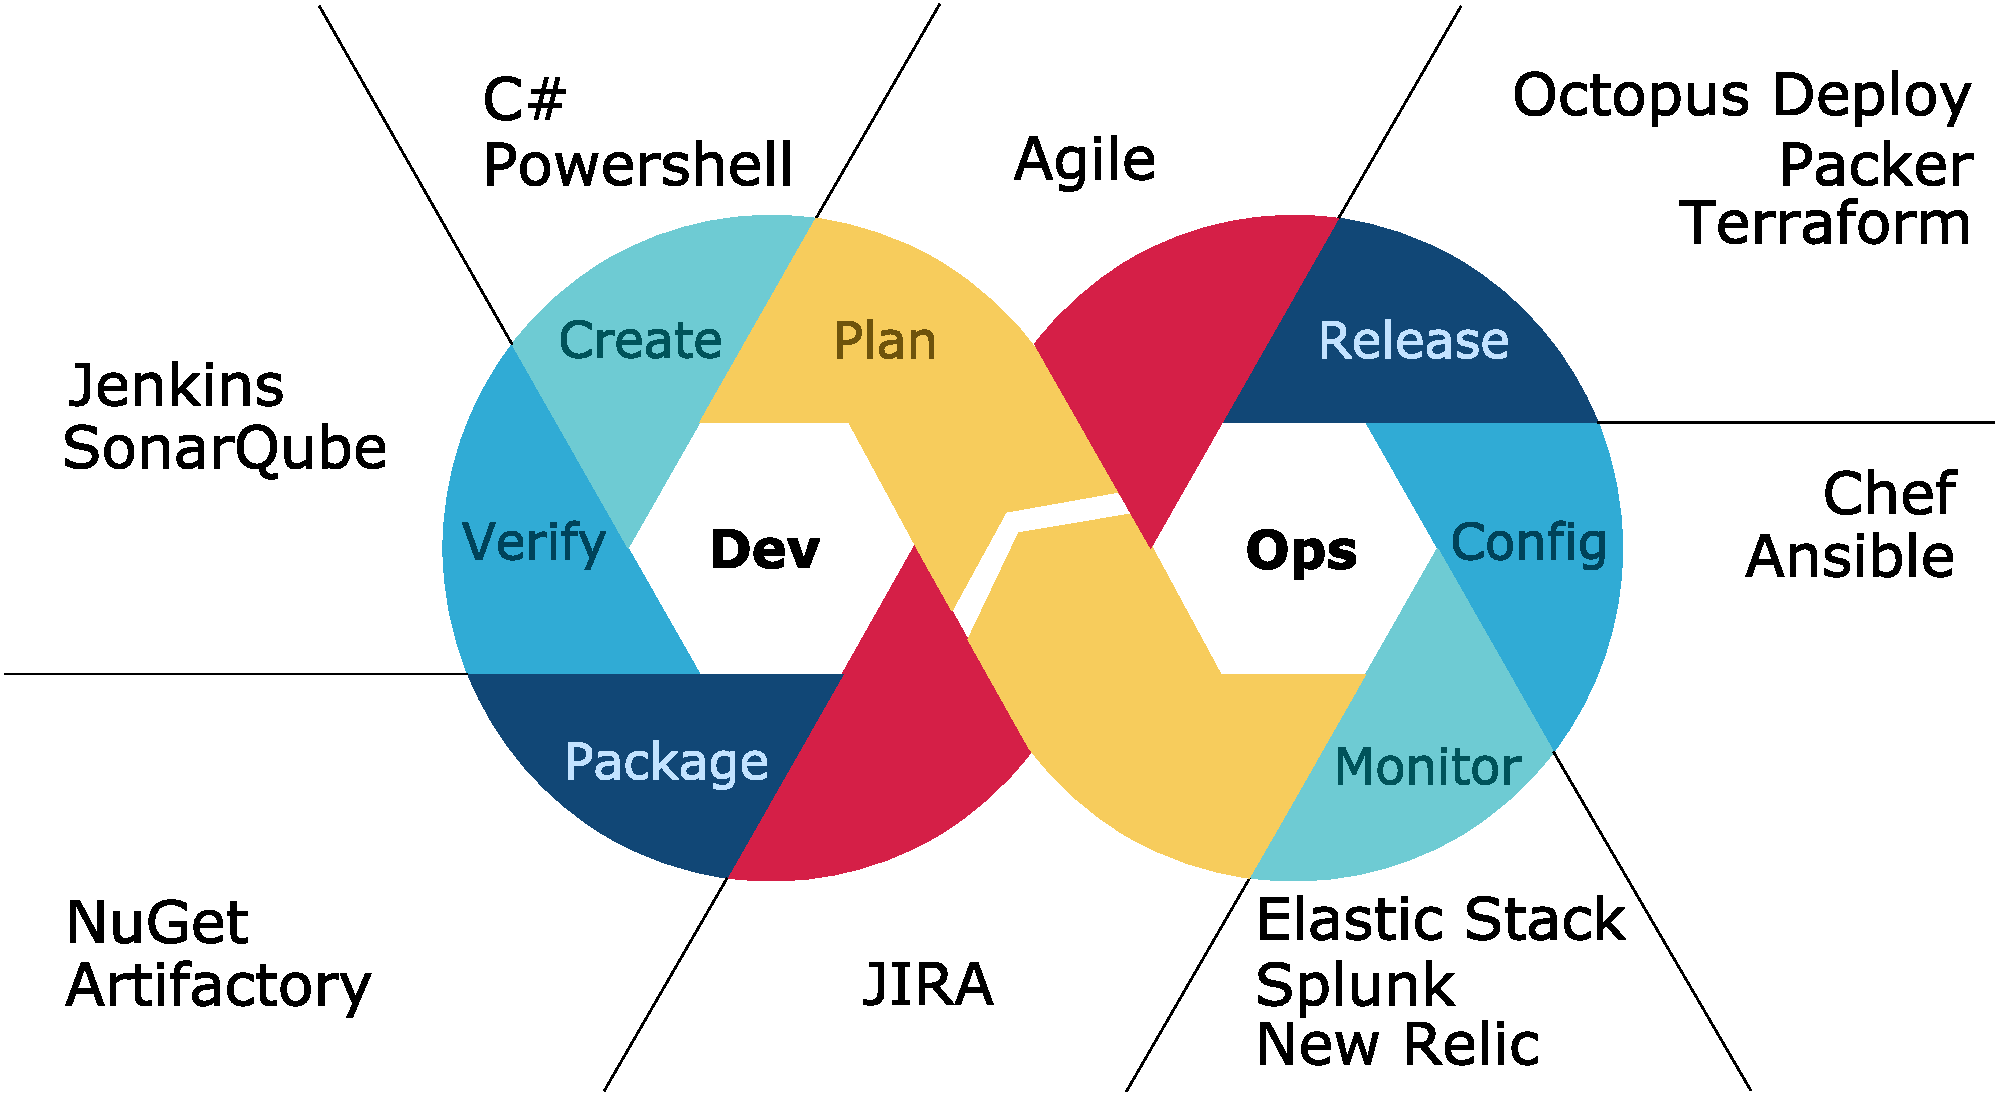
\includegraphics[scale=0.18]{DevOps.pdf}
\vspace{4mm}
}

% Programming skill bars
\programming{{Golang /1}, {Powershell $\textbullet$ Python / 3}, {C $\textbullet$ C++ $\textbullet$ Bash / 3}, {C\# $\textbullet$ SQL $\textbullet$ Entity Framework / 3}}

\iac{{Packer $\textbullet$ Terraform / 3}, {Ansible $\textbullet$ Chef / 3}}

\oses{{Mac OS X / 2}, {Windows $\textbullet$ Linux (Ubuntu) / 3}}

\platforms{{Xbox 360 $\textbullet$ PS3 $\textbullet$ iOS $\textbullet$ Android / 1}, {VMware $\textbullet$ Docker $\textbullet$ Kubernetes / 2}, {AWS / 3}}

\cicd{{Octopus Deploy / 2}, {Jenkins $\textbullet$ GoCD $\textbullet$ Artifactory / 3}}

\monitoring{{Elastic Stack $\textbullet$ Splunk $\textbullet$ New Relic / 2}}

\alerting{{Zabbix $\textbullet$ PagerDuty / 1}}

% Projects text
\projects{
\textbf{\href{http://johnpaulnewman.com/projects/data-pipeline/}{Data Pipeline}}
\begin{itemize}
  \item AWS Lambda (C\# \& Python)
  \item AWS Kinesis
  \item AWS Glue \& Athena
  \item AWS EMR (Scala \& PySpark)
  \item Apache Avro
\end{itemize}
\textbf{\href{http://johnpaulnewman.com/projects/papers-ocr-solution/}{OCR Solution - Hackathon : Winner}}
\begin{itemize}
  \item Python (Flask, Celery, RethinkDB)
  \item RabbitMQ
\end{itemize}
\textbf{\href{http://johnpaulnewman.com/projects/reporting-service/}{Reporting Service}}
\begin{itemize}
  \item C\# (AutoMapper, Windsor, \\ Entity Framework)
  \item JQuery \& d3.js
\end{itemize}
\textbf{\href{http://johnpaulnewman.com/projects/gerrit-backup-solution/}{Gerrit Backup Solution}}
\begin{itemize}
  \item Python
  \item AWS S3
\end{itemize}
\textbf{\href{http://johnpaulnewman.com/projects/csharp-dependencies-graph/}{C\# Dependencies Graph}}
\begin{itemize}
  \item Ruby
  \item Graphviz \& SVG
  \item JQuery
\end{itemize}
\textbf{\href{http://johnpaulnewman.com/projects/chef-lwrp/}{Chef LWRP}}
\begin{itemize}
  \item Chef \& Powershell
\end{itemize}
\textbf{\href{http://johnpaulnewman.com/projects/palm-os-rsrc-extractor/}{Palm OS RSRC Extractor}}
\begin{itemize}
  \item C++, MFC
\end{itemize}
\textbf{\href{http://johnpaulnewman.com/projects/adobe-photoshop-automation/}{Adobe Photoshop Automation}}
\begin{itemize}
  \item C++, COM
\end{itemize}
\textbf{\href{http://johnpaulnewman.com/projects/translation-memory-validation/}{Translation Memory Validation}}
\begin{itemize}
  \item Classic ASP
  \item XSLT with Javascript functions
\end{itemize}
}

\qualifications{
\textbf{Certificate in C++ Programming}\\\textsc{Open University (MT262 Module)\vspace{1.25mm}} \\
\textbf{Certificate in Programming}\\\textsc{Cambridge Information Technology \\(Pascal \& Delphi)\vspace{1.25mm}} \\
\textbf{BTEC 1st Diploma in Science \& Health} \\
12 Distinctions and 4 Merits
}

%----------------------------------------------------------------------------------------
%   PERSONAL INFORMATION
%----------------------------------------------------------------------------------------
% If you don't need one or more of the below, just remove the content leaving the command, e.g. \cvnumberphone{}

\cvname{
  \textbf{JOHN PAUL \vspace{2mm}}\\\textbf{NEWMAN}
} % Your name
\cvjobtitle{Senior Software Engineer \vspace{1.0mm}\\ DevOps} % Job
% title/career

\cvlinkedin{/in/johnpaulnewman} % LinkedIn
\cvgithub{jpnewman} % GitHub
\cvnumberphone{} % Phone number
\cvsite{johnpaulnewman.com} % Personal website
\cvmail{} % Email address

%----------------------------------------------------------------------------------------

\begin{document}

% Stop hyphenation
\hyphenpenalty=10000
\exhyphenpenalty=10000

 % Print the sidebar
\makeprofile

%----------------------------------------------------------------------------------------
%   Summary
%----------------------------------------------------------------------------------------

\section{Summary}

\summary{Senior Software Engineer with  Windows and Linux DevOps experience working in an Agile environment for a FinTech PCI-DSS compliant business. \\
Highly competent in Windows and Linux automation, using Chef and Ansible. \\ Experience in infrastructure automation, using Packer and Terraform, on both Amazon Web Services (AWS) and VMware. Implementation of High Availability (HA) and Disaster Recovery (DR) best practices. \\
Designed and managed Continuous Integration (CI)/Continuous Deployment (CD) tools, processes, and pipelines.}

%----------------------------------------------------------------------------------------
%   EXPERIENCE
%----------------------------------------------------------------------------------------

\section{Work Experience}

\begin{twenty} % Environment for a list with descriptions
%\twentyitem{<date from>}{<date to>}{<title>}{<company>}{<location>}{<description>}{<responsibilities>}{<key achievements>}
\twentyitem
      {2012}% Date From
  {Present} % Date To
    {Senior Software Engineer/DevOps} % Title
    {\href{https://www.wonga.com/}{Wonga}} % Company
    {Ireland - England} % Location
    {Senior Software Engineer with DevOps responsibilities designing, creating and implementing CI/CD tools and infrastructure within a Platform Engineering Team} % Description
  {\begin{itemize}
    \item Implementation and maintenance of AWS infrastructure, including EC2 instances with Active Directory servers
    \item Implementation and maintenance of all CI/CD systems, including Jenkins, Artifactory, Gerrit, Octopus Deploy, and Windows build/deploy agents
    \item Created Ansible playbooks for CI/CD servers
    \item Created HashiCorp Terraform templates to deploy AWS and VMware architecture
    \item Created HashiCorp Packer templates for AWS and VMware
    \item Supported Service Oriented Architecture (SOA) architecture applications that use NServiceBus using both MSMQ with DTC and RabbitMQ transportation layers
    \item Interim Scrum Master and Team Lead
  \end{itemize}
  } % Responsibilities
  {\begin{itemize}
      \item Created Ansible roles to deploy an ELK/Elastic stack, Artifactory, Gerrit, and Jenkins servers
    \item Created a Data pipeline in Python using AWS Lambda, Kinesis, and Glue.
    \item Created a process to deploy a legacy VB6 application using Chef, Powershell, and AWS S3
    \item Developed and maintained Chef Cookbooks for CI servers
    \item Developed a RESTful Reporting Service using C\#, Entity Framework (EF), JQuery and d3.js
    \item Created Powershell build and deploy scripts to replace, Ruby Rake, and MSBuild scripts, which included a DSL implemented in PowerShell for NuGet packing
    \item Developed a Ruby application to create Graphviz DOT files of Microsoft Visual Studio solution dependencies and display them via a JQuery website that allowed selection and filtering
    \item Introduced the use of NuGet, Artifactory, Octopus Deploy to manage dependencies and deployment packages
  \end{itemize}
  } % Key Achievements
\end{twenty}

\newpage
\makeprofiletwo

\section{Work Experience}
\begin{twenty}
\twentyitem
      {2007} % Date From
  {2012} % Date To
    {Software Internationalization Engineer II} % Title
    {\href{https://www.popcap.com/}{PopCap Games International}} % Company
    {Ireland} % Location
    {Worked as one of two internationalization engineers responsible for source code changes to ensure that flagship games, like PopCap's Bejeweled, Plants vs. Zombies, Peggle, and Zuma, worked in multiple regions.} % Description
  {\begin{itemize}
    \item Internationalization and localization of flagship games, across multiple platforms in multiple development languages, including C++ and Objective-C
    \item Liaise with US and APAC project teams to achieve timely delivery and mutual project goals
    \item Act as point of contact/subject matter expert for Internationalization
  \end{itemize}
  } % Responsibilities
  {\begin{itemize}
    \item Managed multiple key projects simultaneously – liaising with multiple project stakeholders in the US and APAC
    \item Developed numerous Python, JavaScript, and VBA tools to reduce engineering time and resources
    \item Reduced art resource requirements by automating Adobe Photoshop to create Asian language Bitmap Fonts
    \item Created a script to import/export text from Photoshop files, allowing for faster translation of graphical assets
    \item Consistently took the initiative to scope and analyze new technology requirements and project impacts
  \end{itemize}
  } % Key Achievements

\end{twenty}

\vspace{0.75\baselineskip}%

\begin{twenty}
\twentyitem
      {2002} % Date From
  {2007} % Date To
    {Software Internationalization and Build Engineer} % Title
    {\href{https://www.welocalize.com/}{Welocalize/Connect Global Solutions}} % Company
    {Ireland} % Location
    {Worked as lead engineer on various projects, responsible for projects and team members.} % Description
  {}
  {\begin{itemize}
    \item Received client recognition for designing, developing and implementing an online system in Classic ASP that validated Translation Memories (TMs) and ensured higher leverage
    \item Created extensive GNU and NMake makefiles
    \item Developed a tool in C++ to extract text from the Palm OS RSRC file format, enabling shorter localization cycles
   \end{itemize}
  }
\end{twenty}

\vspace{0.75\baselineskip}%

\begin{twenty}
\twentyitem
  {2000}
  {2002}
    {Software Localization Engineer}
    {\href{https://www.lionbridge.com/}{Bowne Global Solutions}}
    {Ireland}
    {}
    {}
    {\begin{itemize}
    \item Developed comprehensive functional test scripts for cutting edge mobile device, Handspring VisorPhone
   \end{itemize}
    }
\end{twenty}

\vspace{0.75\baselineskip}%

\begin{twenty}
\twentyitem
  {1998}
  {2000}
    {Software Localization Engineer and IT Network Administrator}
    {Tek Translation}
    {England - Ireland}
    {}
    {}
    {\begin{itemize}
    \item Migrated Novell to Windows NT 4 and Pegasus Mail to Exchange Server
    \item Set-up and maintained Sage Line 100, a MS-DOS based accounting system
   \end{itemize}
    }
\end{twenty}

\end{document}
